\section{Kapacitet} \label{kap}
% Skriv ift kapacitet (ift sengepladser, persona - hvilken betydning har hhv. 95 \% kapacitet mod 105 \%)
Kapacitet omfatter antallet af patienter, kontakter, personale, udstyr og rum. Kontrakter omfatter forundersøgelse, behandling og kontrol. Personalet består af læger, sygeplejersker og sekretærer. Udstyret beskriver de nødvendige maskiner samt antallet af rum der er udstyret med disse. Dette beskriver den samlede kapacitetsudnyttelse som defineres som  mest mulig producering af investerede ressourcer og er forholdet mellem aktivitet og kapacitet. \cite{Company2013} En beskrivelse af dette fremgår af \figref{kapacitet}. 

\begin{figure}[H]
	\flushleft 
	\centering
	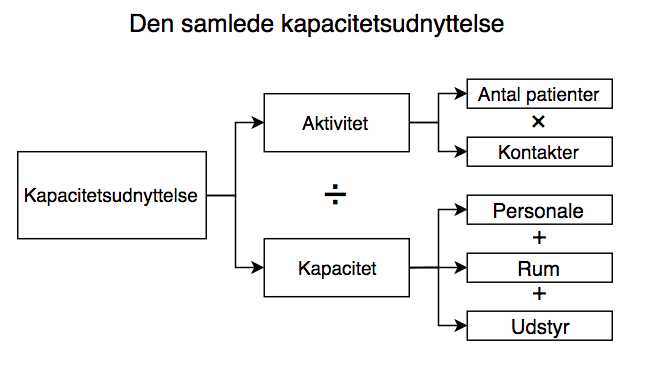
\includegraphics[scale=.45]{figures/Kapacitetsudnyttelse.png}
	\label{kapacitet}
	\flushleft
	\caption{\textit{Flowdiagramet viser den samlede kapacitetsudnyttelse som er opdelt i aktivitet og kapacitet.  \cite{Company2013}}}
\end{figure}


\noindent
Belægning beskriver antallet af patienter, der er normeret til på en afdeling \cite{Heidmann2014}. Når en $100~\%$ belægning opnås svarer dette til at alle sengepladser på en afdeling er taget i brug hvilket er fuld udnyttelse af kapaciteten. Ved en belægningsgrad på over $100~\%$ betyder det, at der er flere patienter end afdelingen er normeret til, hvilket vil sige, at afdelingen yder mere end der er kapacitet til. Ved en belægningsgrad på under $100~\%$ er der omvendt færre patienter end afdelingen er normeret til, således der er tomme sengepladser og afdelingen derved ikke udnytter kapaciteten effektivt. \cite{Pauly1986} 

\subsection{Ortopædkirurgisk afdeling}
Udnyttelsen af kapaciteten afhænger ligeledes af det budget som afdelingen har til rådighed. Dette beløb udregnes ud fra diagnoserelaterede grupper (DRG) systemet. Systemet anvendes til at analysere omkostninger og aktivitet på et hospital.\cite{DRG2016} Ortopædkirurgisk afdelingen har et budget på $700.872.744$ kr, som svarer til 17,2 \% af de samlede budget for alle afdelinger på Aalborg Universitetshospital, hvilket er illusteret af \ref{DRG_budget}.\cite{Rasmussen2016}
Størstedelen af budget anvendes på personale- og patienter udgifter, som svarer til hhv. 60 \% og 32 \%. Det resterende budget anvendes til bygning, it, apparature, inventar samt drift og service. 


\begin{figure}[H]
\flushleft 
	\centering
	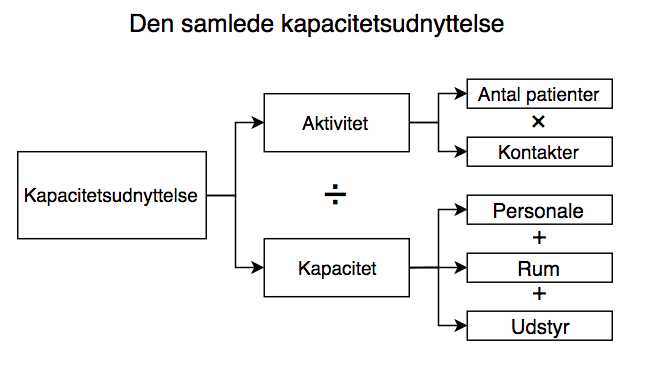
\includegraphics[scale=.45]{figures/Kapacitetsudnyttelse.png}
	\label{kapacitet}
	\flushleft
	\caption{\textit{Flowdiagramet viser den samlede kapacitetsudnyttelse som er inddelt i aktivitet og kapacitet \cite{Company2013}}}
\end{figure}

Afdelingen har XX sengeplader til rådighed som befinder sig på XX afsnit. \fxnote{Vi mangler informationer for at kunne skrive dette færdigt.}

\subsubsection{Udnyttelse af personale} \fxnote{Vi mangler informationer for at kunne skrive dette færdigt.}
% Hvordan opleves belægning generelt på OA på Aalborg UH? Hvordan varetages opgaver af personalet? Hvordan er vagtskifte? Hvor langt tid arbejdes der gennemsnitlig om dagen?
Som beskrevet i \ref{kap} er personalet en af de væsentlige faktorer for at kunne få fuld kapacitetudnyttelse. På ortopædkirurgisk afdeling på Aalborg Universitetshospital arbejder i gennemsnit 37 timer om ugen, hvilket svarer til XX antal timer om dagen. \cite{Danske2015} Under normale omstændigheder varetager sundhedspersonalet XX antal patienter fordelt på XX timer. Afdelingen er delt op i XX antal vagthold og har vagtskifte hver XX time. Personalets opgaver varetages på følgende måder XX. 

\subsubsection{Indlæggelse af patienter}
% Hvordan foregår indlæggelsen på OA på AUH? Hvornår indlæggelses patienterne (elektive patienter) og hvornår på dagen udskrives patienter (både elektive og akutte patienter) Hvor mange patienter hhv. akutte vs. elektive patienter? Hvad er deres buffer i forhold til elektive patienter, således der er plads til de akutte indlæggelser? indkaldes elektive patienter, hvis der er mindre akutte i en periode end der er estimeret til? Øges den normerede kapacitet under overbelægning ved at indkalde vikarbureau? (Altså tager man samme mængde elektive patienter ind.) 

Som beskrevet i \ref{kap} har belægningen en betydning for antallet af normerede senge på en afdeling. Der skal være et sammenspil mellem antal sengepladser og patientindlæggelser. På ortopædkirurgisk afdeling har de XX antal sengepladser til rådighed som er fordelt på XX afsnit. 


Ortopædkirurgisk afdeling tager i gennemsnit XX antal elektive patienter og XX antal akutte patienter ind. Elektive patienter omfatter både indlagte og ambulante patienter, disse skal gennemgå et længerevarende behandlingsforløb. Akuttepatienter defineres, som personer der er henvist til hospitalet som følge af en akut opstået tilstand. Derudover kan elektive patienter med en pludselig forværret tilstand skifte fra en elektiv til akut patient. 
Hvis der sammenlignes med andre afdelinger på Aalborg Universitetshospital er ortopædkirurgisk afdeling den afdeling der har flest elektive indlæggelser, hvilket svarer til $13~\%$ af de samlede indlæggelser. \cite{RegionNord2016}. Elektive patienter indlægges XX på dagen og udskrives igen XX på dagen. Derudover har sundhedspersonalet en 'buffer' i forhold til elektive patienter på XX antal dage for at gøre plads til akutte indlæggelser. Elektive patienter kan derudover tilkaldes hvis antallet af akutte indlæggelser falder over en periode. 